% SOURCE: RG_signed_reanalysis_REFIX20260801.json :: bundles.*.cells.g{2,3,5,10,20}.frac_drop_negative (crossover g per cell; 14B 0.813@2, 1B never crosses)
% !TEX encoding = UTF-8 Unicode
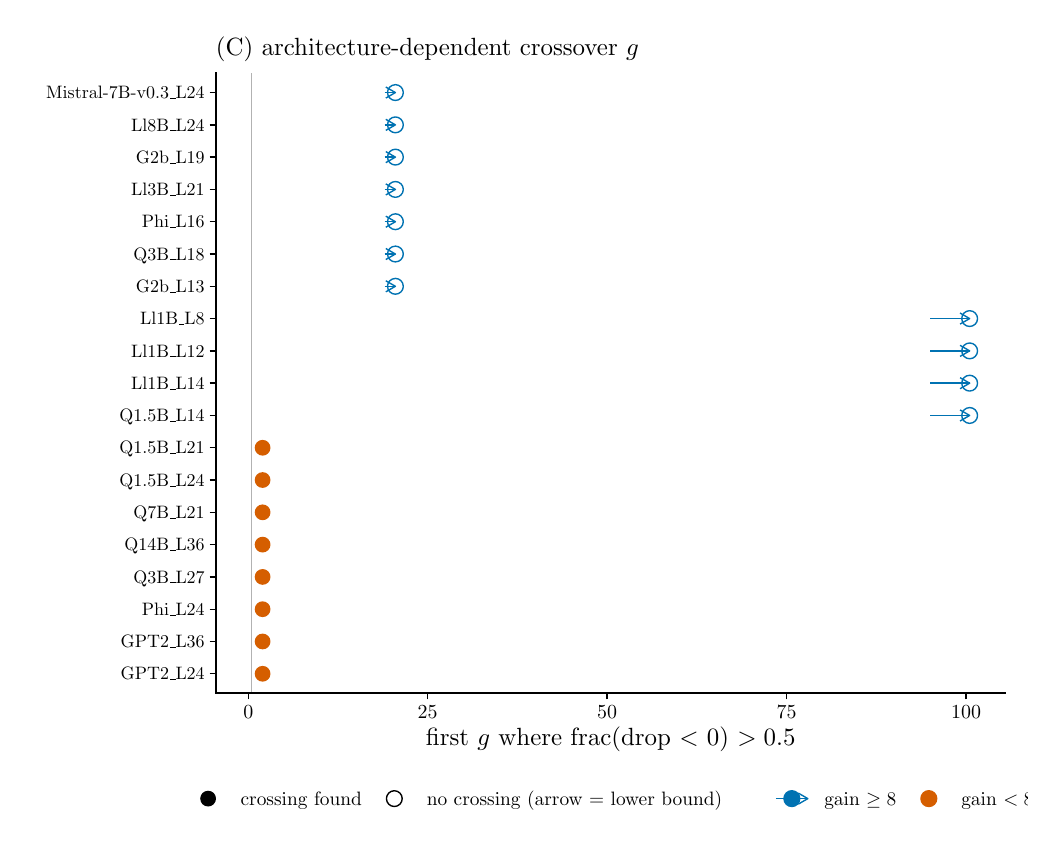
\begin{tikzpicture}[x=1pt,y=1pt]
\definecolor{fillColor}{RGB}{255,255,255}
\path[use as bounding box,fill=fillColor,fill opacity=0.00] (0,0) rectangle (361.35,289.08);
\begin{scope}
\path[clip] (  0.00,  0.00) rectangle (361.35,289.08);
\definecolor{drawColor}{RGB}{255,255,255}
\definecolor{fillColor}{RGB}{255,255,255}

\path[draw=drawColor,line width= 0.5pt,line join=round,line cap=round,fill=fillColor] (  0.00,  0.00) rectangle (361.35,289.08);
\end{scope}
\begin{scope}
\path[clip] ( 68.03, 48.61) rectangle (353.35,272.63);
\definecolor{fillColor}{RGB}{255,255,255}

\path[fill=fillColor] ( 68.03, 48.61) rectangle (353.35,272.63);
\definecolor{drawColor}{gray}{0.70}

\path[draw=drawColor,line width= 0.3pt,line join=round] ( 81.00, 48.61) -- ( 81.00,272.63);
\definecolor{drawColor}{RGB}{0,114,178}

\path[draw=drawColor,line width= 0.5pt,line join=round,line cap=round] (132.88,265.63) circle (  2.85);

\path[draw=drawColor,line width= 0.5pt,line join=round,line cap=round] (132.88,253.96) circle (  2.85);

\path[draw=drawColor,line width= 0.5pt,line join=round,line cap=round] (132.88,242.30) circle (  2.85);

\path[draw=drawColor,line width= 0.5pt,line join=round,line cap=round] (132.88,230.63) circle (  2.85);

\path[draw=drawColor,line width= 0.5pt,line join=round,line cap=round] (132.88,218.96) circle (  2.85);

\path[draw=drawColor,line width= 0.5pt,line join=round,line cap=round] (132.88,207.29) circle (  2.85);

\path[draw=drawColor,line width= 0.5pt,line join=round,line cap=round] (132.88,195.62) circle (  2.85);

\path[draw=drawColor,line width= 0.5pt,line join=round,line cap=round] (340.38,183.96) circle (  2.85);

\path[draw=drawColor,line width= 0.5pt,line join=round,line cap=round] (340.38,172.29) circle (  2.85);

\path[draw=drawColor,line width= 0.5pt,line join=round,line cap=round] (340.38,160.62) circle (  2.85);

\path[draw=drawColor,line width= 0.5pt,line join=round,line cap=round] (340.38,148.95) circle (  2.85);
\definecolor{fillColor}{RGB}{213,94,0}

\path[fill=fillColor] ( 84.89,137.28) circle (  2.85);

\path[fill=fillColor] ( 84.89,125.62) circle (  2.85);

\path[fill=fillColor] ( 84.89,113.95) circle (  2.85);

\path[fill=fillColor] ( 84.89,102.28) circle (  2.85);

\path[fill=fillColor] ( 84.89, 90.61) circle (  2.85);

\path[fill=fillColor] ( 84.89, 78.94) circle (  2.85);

\path[fill=fillColor] ( 84.89, 67.28) circle (  2.85);

\path[fill=fillColor] ( 84.89, 55.61) circle (  2.85);

\path[draw=drawColor,line width= 0.5pt,line join=round] (128.99,265.63) -- (132.88,265.63);

\path[draw=drawColor,line width= 0.5pt,line join=round] (129.41,263.63) --
	(132.88,265.63) --
	(129.41,267.63);

\path[draw=drawColor,line width= 0.5pt,line join=round] (128.99,253.96) -- (132.88,253.96);

\path[draw=drawColor,line width= 0.5pt,line join=round] (129.41,251.96) --
	(132.88,253.96) --
	(129.41,255.96);

\path[draw=drawColor,line width= 0.5pt,line join=round] (128.99,242.30) -- (132.88,242.30);

\path[draw=drawColor,line width= 0.5pt,line join=round] (129.41,240.30) --
	(132.88,242.30) --
	(129.41,244.30);

\path[draw=drawColor,line width= 0.5pt,line join=round] (128.99,230.63) -- (132.88,230.63);

\path[draw=drawColor,line width= 0.5pt,line join=round] (129.41,228.63) --
	(132.88,230.63) --
	(129.41,232.63);

\path[draw=drawColor,line width= 0.5pt,line join=round] (128.99,218.96) -- (132.88,218.96);

\path[draw=drawColor,line width= 0.5pt,line join=round] (129.41,216.96) --
	(132.88,218.96) --
	(129.41,220.96);

\path[draw=drawColor,line width= 0.5pt,line join=round] (128.99,207.29) -- (132.88,207.29);

\path[draw=drawColor,line width= 0.5pt,line join=round] (129.41,205.29) --
	(132.88,207.29) --
	(129.41,209.29);

\path[draw=drawColor,line width= 0.5pt,line join=round] (128.99,195.62) -- (132.88,195.62);

\path[draw=drawColor,line width= 0.5pt,line join=round] (129.41,193.62) --
	(132.88,195.62) --
	(129.41,197.62);

\path[draw=drawColor,line width= 0.5pt,line join=round] (326.12,183.96) -- (340.38,183.96);

\path[draw=drawColor,line width= 0.5pt,line join=round] (336.92,181.96) --
	(340.38,183.96) --
	(336.92,185.96);

\path[draw=drawColor,line width= 0.5pt,line join=round] (326.12,172.29) -- (340.38,172.29);

\path[draw=drawColor,line width= 0.5pt,line join=round] (336.92,170.29) --
	(340.38,172.29) --
	(336.92,174.29);

\path[draw=drawColor,line width= 0.5pt,line join=round] (326.12,160.62) -- (340.38,160.62);

\path[draw=drawColor,line width= 0.5pt,line join=round] (336.92,158.62) --
	(340.38,160.62) --
	(336.92,162.62);

\path[draw=drawColor,line width= 0.5pt,line join=round] (326.12,148.95) -- (340.38,148.95);

\path[draw=drawColor,line width= 0.5pt,line join=round] (336.92,146.95) --
	(340.38,148.95) --
	(336.92,150.95);
\end{scope}
\begin{scope}
\path[clip] (  0.00,  0.00) rectangle (361.35,289.08);
\definecolor{drawColor}{RGB}{0,0,0}

\path[draw=drawColor,line width= 0.5pt,line join=round,line cap=rect] ( 68.03, 48.61) --
	( 68.03,272.63);
\end{scope}
\begin{scope}
\path[clip] (  0.00,  0.00) rectangle (361.35,289.08);
\definecolor{drawColor}{RGB}{0,0,0}

\node[text=drawColor,anchor=base east,inner sep=0pt, outer sep=0pt, scale=  0.65] at ( 63.98, 53.37) {GPT2\_L24};

\node[text=drawColor,anchor=base east,inner sep=0pt, outer sep=0pt, scale=  0.65] at ( 63.98, 65.04) {GPT2\_L36};

\node[text=drawColor,anchor=base east,inner sep=0pt, outer sep=0pt, scale=  0.65] at ( 63.98, 76.70) {Phi\_L24};

\node[text=drawColor,anchor=base east,inner sep=0pt, outer sep=0pt, scale=  0.65] at ( 63.98, 88.37) {Q3B\_L27};

\node[text=drawColor,anchor=base east,inner sep=0pt, outer sep=0pt, scale=  0.65] at ( 63.98,100.04) {Q14B\_L36};

\node[text=drawColor,anchor=base east,inner sep=0pt, outer sep=0pt, scale=  0.65] at ( 63.98,111.71) {Q7B\_L21};

\node[text=drawColor,anchor=base east,inner sep=0pt, outer sep=0pt, scale=  0.65] at ( 63.98,123.38) {Q1.5B\_L24};

\node[text=drawColor,anchor=base east,inner sep=0pt, outer sep=0pt, scale=  0.65] at ( 63.98,135.04) {Q1.5B\_L21};

\node[text=drawColor,anchor=base east,inner sep=0pt, outer sep=0pt, scale=  0.65] at ( 63.98,146.71) {Q1.5B\_L14};

\node[text=drawColor,anchor=base east,inner sep=0pt, outer sep=0pt, scale=  0.65] at ( 63.98,158.38) {Ll1B\_L14};

\node[text=drawColor,anchor=base east,inner sep=0pt, outer sep=0pt, scale=  0.65] at ( 63.98,170.05) {Ll1B\_L12};

\node[text=drawColor,anchor=base east,inner sep=0pt, outer sep=0pt, scale=  0.65] at ( 63.98,181.72) {Ll1B\_L8};

\node[text=drawColor,anchor=base east,inner sep=0pt, outer sep=0pt, scale=  0.65] at ( 63.98,193.38) {G2b\_L13};

\node[text=drawColor,anchor=base east,inner sep=0pt, outer sep=0pt, scale=  0.65] at ( 63.98,205.05) {Q3B\_L18};

\node[text=drawColor,anchor=base east,inner sep=0pt, outer sep=0pt, scale=  0.65] at ( 63.98,216.72) {Phi\_L16};

\node[text=drawColor,anchor=base east,inner sep=0pt, outer sep=0pt, scale=  0.65] at ( 63.98,228.39) {Ll3B\_L21};

\node[text=drawColor,anchor=base east,inner sep=0pt, outer sep=0pt, scale=  0.65] at ( 63.98,240.06) {G2b\_L19};

\node[text=drawColor,anchor=base east,inner sep=0pt, outer sep=0pt, scale=  0.65] at ( 63.98,251.72) {Ll8B\_L24};

\node[text=drawColor,anchor=base east,inner sep=0pt, outer sep=0pt, scale=  0.65] at ( 63.98,263.39) {Mistral-7B-v0.3\_L24};
\end{scope}
\begin{scope}
\path[clip] (  0.00,  0.00) rectangle (361.35,289.08);
\definecolor{drawColor}{RGB}{0,0,0}

\path[draw=drawColor,line width= 0.5pt,line join=round] ( 65.78, 55.61) --
	( 68.03, 55.61);

\path[draw=drawColor,line width= 0.5pt,line join=round] ( 65.78, 67.28) --
	( 68.03, 67.28);

\path[draw=drawColor,line width= 0.5pt,line join=round] ( 65.78, 78.94) --
	( 68.03, 78.94);

\path[draw=drawColor,line width= 0.5pt,line join=round] ( 65.78, 90.61) --
	( 68.03, 90.61);

\path[draw=drawColor,line width= 0.5pt,line join=round] ( 65.78,102.28) --
	( 68.03,102.28);

\path[draw=drawColor,line width= 0.5pt,line join=round] ( 65.78,113.95) --
	( 68.03,113.95);

\path[draw=drawColor,line width= 0.5pt,line join=round] ( 65.78,125.62) --
	( 68.03,125.62);

\path[draw=drawColor,line width= 0.5pt,line join=round] ( 65.78,137.28) --
	( 68.03,137.28);

\path[draw=drawColor,line width= 0.5pt,line join=round] ( 65.78,148.95) --
	( 68.03,148.95);

\path[draw=drawColor,line width= 0.5pt,line join=round] ( 65.78,160.62) --
	( 68.03,160.62);

\path[draw=drawColor,line width= 0.5pt,line join=round] ( 65.78,172.29) --
	( 68.03,172.29);

\path[draw=drawColor,line width= 0.5pt,line join=round] ( 65.78,183.96) --
	( 68.03,183.96);

\path[draw=drawColor,line width= 0.5pt,line join=round] ( 65.78,195.62) --
	( 68.03,195.62);

\path[draw=drawColor,line width= 0.5pt,line join=round] ( 65.78,207.29) --
	( 68.03,207.29);

\path[draw=drawColor,line width= 0.5pt,line join=round] ( 65.78,218.96) --
	( 68.03,218.96);

\path[draw=drawColor,line width= 0.5pt,line join=round] ( 65.78,230.63) --
	( 68.03,230.63);

\path[draw=drawColor,line width= 0.5pt,line join=round] ( 65.78,242.30) --
	( 68.03,242.30);

\path[draw=drawColor,line width= 0.5pt,line join=round] ( 65.78,253.96) --
	( 68.03,253.96);

\path[draw=drawColor,line width= 0.5pt,line join=round] ( 65.78,265.63) --
	( 68.03,265.63);
\end{scope}
\begin{scope}
\path[clip] (  0.00,  0.00) rectangle (361.35,289.08);
\definecolor{drawColor}{RGB}{0,0,0}

\path[draw=drawColor,line width= 0.5pt,line join=round,line cap=rect] ( 68.03, 48.61) --
	(353.35, 48.61);
\end{scope}
\begin{scope}
\path[clip] (  0.00,  0.00) rectangle (361.35,289.08);
\definecolor{drawColor}{RGB}{0,0,0}

\path[draw=drawColor,line width= 0.5pt,line join=round] ( 79.71, 46.36) --
	( 79.71, 48.61);

\path[draw=drawColor,line width= 0.5pt,line join=round] (144.55, 46.36) --
	(144.55, 48.61);

\path[draw=drawColor,line width= 0.5pt,line join=round] (209.39, 46.36) --
	(209.39, 48.61);

\path[draw=drawColor,line width= 0.5pt,line join=round] (274.24, 46.36) --
	(274.24, 48.61);

\path[draw=drawColor,line width= 0.5pt,line join=round] (339.08, 46.36) --
	(339.08, 48.61);
\end{scope}
\begin{scope}
\path[clip] (  0.00,  0.00) rectangle (361.35,289.08);
\definecolor{drawColor}{RGB}{0,0,0}

\node[text=drawColor,anchor=base,inner sep=0pt, outer sep=0pt, scale=  0.72] at ( 79.71, 39.60) {0};

\node[text=drawColor,anchor=base,inner sep=0pt, outer sep=0pt, scale=  0.72] at (144.55, 39.60) {25};

\node[text=drawColor,anchor=base,inner sep=0pt, outer sep=0pt, scale=  0.72] at (209.39, 39.60) {50};

\node[text=drawColor,anchor=base,inner sep=0pt, outer sep=0pt, scale=  0.72] at (274.24, 39.60) {75};

\node[text=drawColor,anchor=base,inner sep=0pt, outer sep=0pt, scale=  0.72] at (339.08, 39.60) {100};
\end{scope}
\begin{scope}
\path[clip] (  0.00,  0.00) rectangle (361.35,289.08);
\definecolor{drawColor}{RGB}{0,0,0}

\node[text=drawColor,anchor=base,inner sep=0pt, outer sep=0pt, scale=  0.90] at (210.69, 29.75) {first $g$ where frac(drop $<$ 0) $> 0.5$};
\end{scope}
\begin{scope}
\path[clip] (  0.00,  0.00) rectangle (361.35,289.08);
\definecolor{fillColor}{RGB}{255,255,255}

\path[fill=fillColor] ( 53.47,  2.00) rectangle (255.40, 19.00);
\end{scope}
\begin{scope}
\path[clip] (  0.00,  0.00) rectangle (361.35,289.08);
\definecolor{fillColor}{RGB}{255,255,255}

\path[fill=fillColor] ( 57.97,  6.50) rectangle ( 72.43, 14.50);
\definecolor{fillColor}{RGB}{0,0,0}

\path[fill=fillColor] ( 65.20, 10.50) circle (  2.85);
\end{scope}
\begin{scope}
\path[clip] (  0.00,  0.00) rectangle (361.35,289.08);
\definecolor{fillColor}{RGB}{255,255,255}

\path[fill=fillColor] (125.26,  6.50) rectangle (139.72, 14.50);
\definecolor{drawColor}{RGB}{0,0,0}

\path[draw=drawColor,line width= 0.5pt,line join=round,line cap=round] (132.49, 10.50) circle (  2.85);
\end{scope}
\begin{scope}
\path[clip] (  0.00,  0.00) rectangle (361.35,289.08);
\definecolor{drawColor}{RGB}{0,0,0}

\node[text=drawColor,anchor=base west,inner sep=0pt, outer sep=0pt, scale=  0.70] at ( 76.93,  8.09) {crossing found};
\end{scope}
\begin{scope}
\path[clip] (  0.00,  0.00) rectangle (361.35,289.08);
\definecolor{drawColor}{RGB}{0,0,0}

\node[text=drawColor,anchor=base west,inner sep=0pt, outer sep=0pt, scale=  0.70] at (144.22,  8.09) {no crossing (arrow = lower bound)};
\end{scope}
\begin{scope}
\path[clip] (  0.00,  0.00) rectangle (361.35,289.08);
\definecolor{fillColor}{RGB}{255,255,255}

\path[fill=fillColor] (264.40,  2.00) rectangle (367.91, 19.00);
\end{scope}
\begin{scope}
\path[clip] (  0.00,  0.00) rectangle (361.35,289.08);
\definecolor{fillColor}{RGB}{255,255,255}

\path[fill=fillColor] (268.90,  6.50) rectangle (283.35, 14.50);
\definecolor{drawColor}{RGB}{0,114,178}
\definecolor{fillColor}{RGB}{0,114,178}

\path[draw=drawColor,line width= 0.5pt,line join=round,line cap=round,fill=fillColor] (276.13, 10.50) circle (  2.85);

\path[draw=drawColor,line width= 0.5pt,line join=round] (270.35, 10.50) -- (281.91, 10.50);

\path[draw=drawColor,line width= 0.5pt,line join=round] (278.44,  8.50) --
	(281.91, 10.50) --
	(278.44, 12.50);
\end{scope}
\begin{scope}
\path[clip] (  0.00,  0.00) rectangle (361.35,289.08);
\definecolor{fillColor}{RGB}{255,255,255}

\path[fill=fillColor] (318.41,  6.50) rectangle (332.86, 14.50);
\definecolor{drawColor}{RGB}{213,94,0}
\definecolor{fillColor}{RGB}{213,94,0}

\path[draw=drawColor,line width= 0.5pt,line join=round,line cap=round,fill=fillColor] (325.63, 10.50) circle (  2.85);
\end{scope}
\begin{scope}
\path[clip] (  0.00,  0.00) rectangle (361.35,289.08);
\definecolor{drawColor}{RGB}{0,0,0}

\node[text=drawColor,anchor=base west,inner sep=0pt, outer sep=0pt, scale=  0.70] at (287.85,  8.09) {gain $\geq 8$};
\end{scope}
\begin{scope}
\path[clip] (  0.00,  0.00) rectangle (361.35,289.08);
\definecolor{drawColor}{RGB}{0,0,0}

\node[text=drawColor,anchor=base west,inner sep=0pt, outer sep=0pt, scale=  0.70] at (337.36,  8.09) {gain $< 8$};
\end{scope}
\begin{scope}
\path[clip] (  0.00,  0.00) rectangle (361.35,289.08);
\definecolor{drawColor}{RGB}{0,0,0}

\node[text=drawColor,anchor=base west,inner sep=0pt, outer sep=0pt, scale=  0.90] at ( 68.03,278.88) {(C) architecture-dependent crossover $g$};
\end{scope}
\end{tikzpicture}
